%%%%%%%%%%%%%%%%%%%%%%%%%%%%%%%%%
% Laatste aanpassing:
%
% 9/4/11 [Greetje]: volledige herwerking
%
% 11/1/2003 [Jan]: label chap:rijen bijgevoegd
%
% 19/9/02 [Jan]: meervoudig gedefinieerde labels (eq:vb1 enzo 
%	veranderd in eq:voorb1 enz...)
%
% 9/9/02 [Jan]:
%           
% 10/09/01 door Greetje
%   typfouten Roby verbeterd
%   titels een klein beetje aangepast owv uniformiteit
%   \vspace{0.3cm} tussen caption en tabel
%   \newpage op lijn 681
%
% 01/09/01 door Greetje          
%%%%%%%%%%%%%%%%%%%%%%%%%%%%%%%%%




\newsavebox{\boog}
\setlength{\unitlength}{1mm}

\chapter{Rijen en financi\"{e}le toepassingen}\label{chap:rijen}

\begin{quote}
     \textit{{\small `En hoeveel uur les hadden jullie per dag?' zei
     Alice, die vlug van onderwerp wilde veranderen.}}

     \textit{{\small `De eerste dag tien uur,' zei de Nepschildpad,
     `de volgende negen enzovoort.'}}

     \textit{{\small `Wat een raar lesrooster!' riep Alice uit.}}

     \textit{{\small `Zo lesten we onze dorst naar kennis steeds
     sneller,' merkte de Griffioen op, `vandaar de uitdrukking ''lest
     best''.'}}

     \textit{{\small Dat was volkomen nieuw voor Alice en ze dacht er
     even over na voordat ze haar volgende opmerking maakte. `Dus
     hadden jullie de elfde dag vrij?'}}

     \textit{{\small `Reken maar,' zei de Nepschildpad.}}

     \textit{{\small `En wat deden jullie met de twaalfde dag?' vroeg
     Alice gretig verder.}}

          Uit `Alice in Wonderland' -- Lewis Carroll
\end{quote}



\newpage
\section{Rijen: definitie en voorbeelden}

Bekijk de volgende opsommingen van getallen:
\begin{eqnarray}
     & -1 ,3 , 7, -5 , -9&
    \label{eq:voorb1}  \\
     & -8,-5,-2,1,4 &
    \label{eq:voorb2} \label{vb2}  \\
     & -\dfrac{1}{4},\dfrac{1}{8},-\dfrac{1}{16},\dfrac{1}{32} &
    \label{eq:voorb3}  \\
     & -1,-2,-5,-14,-41&
    \label{eq:voorb4}
\end{eqnarray}

Voor elke opsomming kunnen we aan ieder getal een rangnummer
toekennen: 1 voor het eerste getal, 2 voor het tweede getal,\ldots\ Dit
rangnummer is vanzelfsprekend een natuurlijk getal. Wanneer er een
dergelijke rangschikking is bij een opsomming van getallen,
spreken we van een \textit{rij} getallen. 

Bekijk de rijen
(\ref{eq:voorb1})
t.e.m. (\ref{eq:voorb4}). Je
merkt op dat we sommige rijen verder kunnen aanvullen omdat er een patroon, een
formule of een verband tussen een element van de rij en het
volgende element bestaat.
\begin{itemize}
    \item  Rij (\ref{eq:voorb2}) gaat verder met  $7$ want men telt
telkens 3 eenheden op  bij het vorige element.

    \item  Bij rij (\ref{eq:voorb3}) merken we op dat de elementen
    afwisselend positief en negatief zijn.
De noemers  schrijven we als opeenvolgende machten van 2, waarbij we
ontdekken dat elk element uit het vorige te berekenen valt door te
vermenigvuldigen met factor $-\frac{1}{2}$. Het volgende element in de rij is dus het getal $-\frac{1}{64}$.
\item In de eerste rij (\ref{eq:voorb1}) is er \emph{geen} structuur terug te vinden (alhoewel, als je maar lang genoeg zoekt vind je ooit wel eens een regelmaat in de rij \ldots).
\item De laatste rij (\ref{eq:voorb4}) is een moeilijke. Het volgend element van de rij vind je als je het vorige element vermenigvuldigt  met 3 en er 1 bij optelt.
\end{itemize}

In wat volgt defini\"eren we het begrip `rij' en geven we enkele voorbeelden.


\subsection{Definitie}


\begin{quote}
    Een rij is \emph{een opsomming van  getallen die in een bepaalde volgorde voorkomen}. Elk element van de rij heeft zijn vaste plaats. In het algemeen noteren we een rij als volgt:
    \[
    t_1, t_2, t_3, \dots
    \]
    Elk element heeft een volgnummer, dat we \textit{index} noemen. De elementen van een rij noemen we de \textit{termen} van de rij. Een rij kan een eindig of een oneindig aantal termen bevatten. 
    \end{quote}
Soms is er een patroon tussen elementen, maar dat is niet altijd het geval. In secties \ref{sec:RR} en \ref{sec:MR} gaan we dieper in op twee soorten patronen die veel voorkomen. Maar eerst geven we enkele voorbeelden.


\subsection{Voorbeelden}
\label{subsec:voorbeelden_rijen}
\subsubsection*{Konijnenrij}
\begin{figure}[htbp]
\centering
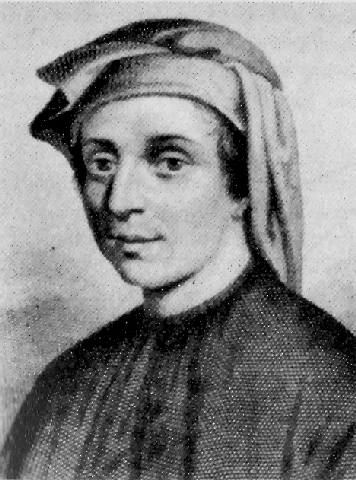
\includegraphics[scale=1]{figuren/rijen/Fibonacci.jpg} 
\caption{Leonardo van Pisa a.k.a Fibonacci ca. 1170--ca. 1250}
\end{figure}
Leonardo Fibonacci was een wiskundige die rond 1200 leefde. Hij stelde volgend probleem:
\begin{quote}
Een konijnenpaar begint zich twee maanden na de geboorte voort te planten en werpt van dan af maandelijks een nieuw konijnenpaar. De nakomelingen planten zich op dezelfde manier voort. Hoeveel konijnenparen zijn er na $n$ maanden?
\end{quote}

Fibonacci rekende uit dat het aantal aanwezige konijnenparen in een maand gelijk is aan 1, 1, 2, 3, 5, 8, 13, 21, 34, 55, \dots  \ We noemen deze rij de `rij van Fibonacci' ofwel de `Konijnenrij'.


\subsubsection*{Enkelvoudige intrest}
\begin{quote}
    We zetten een kapitaal van \euros{10\,000} op een spaarboekje met
    jaarlijkse intrest van \SI{6}{\percent}. Wat zijn de kapitalen jaar
    na jaar  tegen enkelvoudige intrest, d.w.z.\ de intrest
    wordt steeds berekend op het beginkapitaal?
\end{quote}
\label{page:intrest}
De groei van het gespaarde kapitaal (kapitaal plus intrest) jaar na jaar vind je in tabel~\ref{tbl:enkelv_intrest}. `Enkelvoudig intrest' kan je je als volgt voorstellen: je laat het beginbedrag op de rekening staan, maar de intrest neem je elk jaar mee naar huis.

\begin{table}[htb]
    \centering
    \caption{Gespaarde kapitaal bij enkelvoudige intrest per jaar}
    \begin{tabular}{cccc}
    \toprule
    jaar & & gespaarde kapitaal & \\
    \midrule
    0  	& $k_0$		&	\num{10000}	&	\\
    1	&	$k_1$	&	\num{10600}	&	$+600$\\
    2	&	$k_2$	&	\num{11200}	&	$+600$\\
    3	&	$k_3$	&	\num{11800}	&	$+600$\\
    \bottomrule
     \end{tabular}
    \label{tbl:enkelv_intrest}
\end{table}

De getallen in de derde kolom vormen een opsomming van  getallen die in een bepaalde volgorde voorkomen. Het is een \emph{rij}. Het gespaarde kapitaal bij enkelvoudige intrest per jaar is dus een rij $k_i$ waarbij $i$ aangeeft welk jaar het betreft. Met het eerste element $k_0$ doelen we op het beginkapitaal. Ieder element kan berekend worden uit het voorgaande element door er 600 bij op te tellen (figuur~\ref{fig:enkelvintrest1}).
\begin{figure}[htbp]
    \centering
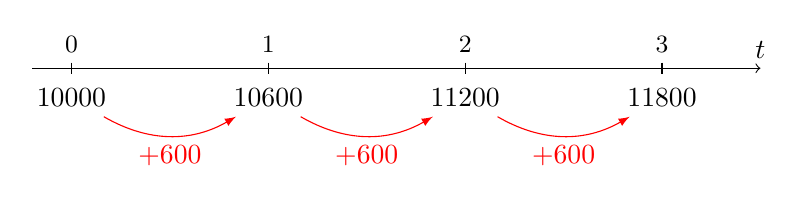
\begin{tikzpicture}[x=2.5cm]
\draw[->] (-0.2,0) -- (3.5,0) node [at end, above] {$t$};
\foreach \x/\y in {0/\num{10000},1/\num{10600},2/\num{11200},3/\num{11800}}{
	\draw[shift={(\x,0.0)}] (0pt,2pt) -- (0pt,-2pt) node[above=4pt] {\small $\x$};
	\node (\x) [below=4pt] at (\x,0) {\y};
}
\foreach \x/\y in {0/1,1/2,2/3}
	\draw[-latex,red] (\x) to [bend right]  node [below] {$+600$} (\y);
\end{tikzpicture}
    \caption{Groei van kapitaal van \euros{10\,000}, \emph{enkelvoudige} intrest van \SI{6}{\percent}}
    \label{fig:enkelvintrest1} 
\end{figure}

\subsubsection*{Samengestelde intrest}
\begin{quote}
   We zetten opnieuw een kapitaal van \euros{10\,000} op een spaarboekje met
    jaarlijkse intrest van \SI{6}{\percent}. Wat zijn de kapitalen jaar
    na jaar tegen samengestelde intrest, waarbij de intrest telkens bij het vorige
    kapitaal opgeteld wordt zodat die mee intrest kan opbrengen?
\end{quote}

We stellen opnieuw een tabel op (tabel~\ref{tbl:samengest_intrest}). De getallen in de derde kolom zijn weer een rij. Het gespaarde kapitaal bij samengestelde intrest per jaar is een rij $m_i$. Het getal $m_0$ is het beginkapitaal. Ieder element kan berekend worden uit het voorgaande element door het te vermenigvuldigen met \num{1.06}.

\begin{table}[htb]
    \centering
    \caption{Gespaarde kapitaal bij samengestelde intrest per jaar}
    \begin{tabular}{cccc}
    \toprule
    jaar & & gespaarde kapitaal & \\
    \midrule
    0  	& 	$m_0$		&	$10\,000$	&	\\
    1	&	$m_1$	&	$\num{10000}+\num{0,06}\cdot\num{10000}=\num{10600}$	&	$\cdot \num{1.06}$\\
    2	&	$m_2$	&	$\num{10600}+\num{0,06}\cdot\num{10600}=\num{11236}$	&	$\cdot \num{1.06}$\\
    3	&	$m_3$	&	$\num{11236}+\num{0,06}\cdot\num{11236}=\num{11910.16}$	&	$\cdot \num{1.06}$\\
    \bottomrule
     \end{tabular}
    \label{tbl:samengest_intrest}
\end{table}


\begin{figure}[htbp]
    \centering
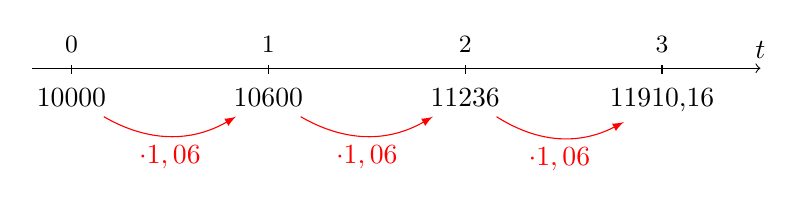
\begin{tikzpicture}[x=2.5cm]
\draw[->] (-0.2,0) -- (3.5,0) node [at end, above] {$t$};
\foreach \x/\y in {0/\num{10000},1/\num{10600},2/\num{11236},3/\num{11910,16}}{
	\draw[shift={(\x,0.0)}] (0pt,1pt) -- (0pt,-2pt) node[above=4pt] {\small $\x$};
	\node (\x) [below=4pt] at (\x,0) {\y};
}
\foreach \x/\y in {0/1,1/2,2/3}
	\draw[-latex,red] (\x) to [bend right]  node [below] {$\cdot \num{1,06}$} (\y);
\end{tikzpicture}
    \caption{Groei van kapitaal van \euros{10\,000}, \emph{samengestelde} intrest van \SI{6}{\percent}}
    \label{fig:enkelvintrest} 
\end{figure}

\section{Rekenkundige rij}
\label{sec:RR}
In het tweede voorbeeld van sectie~\ref{subsec:voorbeelden_rijen} (enkelvoudige intrest) hebben we gezien dat 
het gespaarde kapitaal bij enkelvoudige intrest per jaar een rij $k_i$ is met een specifiek patroon:  ieder element kan berekend worden uit het voorgaande element door er 600 bij op te tellen.

Dit patroon komt vaak voor bij rijen en
krijgt daarom de speciale naam \textit{rekenkundige rij}. De definitie
van rekenkundige rij is de volgende:


\subsection{Definitie}
\begin{quote}
Een rekenkundige rij is \emph{een rij waarbij elke term de som is van de vorige term en een constant getal $v$ (het verschil van de rij).}
\end{quote}
\begin{displaymath}
   t_1, t_2, t_3, \dots  \mbox{ is een \emph{rekenkundige
    rij}}
\end{displaymath}
\begin{displaymath}
    \Updownarrow
\end{displaymath}
\begin{displaymath}
    t_{2}-t_{1}=t_{3}-t_{2}=\dots=t_{n}-t_{n-1} =v
\end{displaymath}

Uit deze definitie leiden we af dat een rekenkundige rij volledig bepaald is door het verschil $v$ en het eerste element van de rij. Omdat $t_n=t_{n-1}+v$, is het $n$-de element van de rij gegeven door 
    \begin{equation}
        t_{n}=t_{1}+(n-1)\cdot v
        \label{eq:algelementrr}
    \end{equation}
Het verschil $v$ kunnen we berekenen als we twee willekeurige elementen van de rij kennen met hun rangnummer:
\[
  t_{n}=t_{u}+(n-u)\cdot v
\]

\subsection{Som van elementen van een een rekenkundige rij}
In heel wat toepassingen komt de \emph{som
van opeenvolgende elementen van een rekenkundige rij} voor.  Een dergelijke som
noemen we \emph{par\-tieel\-som} en noteren we door $S_{n}$,
waarbij $n$ duidt op het \emph{aantal} termen in de som. Omwille van het specifieke verband tussen de termen van de som, kunnen we een formule zoeken voor $S_{n}$.

We schrijven de som van die $n$ termen op 2 manieren op: van links naar
rechts en omgekeerd. We tellen lid aan lid op.
\begin{displaymath}
    \begin{array}{ccccccccccc}
    S_{n} & = & t_{1} & + & t_{2} & + & t_{3} & + &
    \ldots & + & t_{n}  \\
    S_{n} & = & t_{n} & + & t_{n-1} & + & t_{n-2} & + &
    \ldots & + & t_{1}  \\
    \hline
    2\cdot S_{n} & = & (t_{1}+t_{n}) & + & (t_{2}+t_{n-1}) & + &
    (t_{3}+t_{n-2}) & + & \ldots & + & (t_{n}+t_{1})
\end{array}
\end{displaymath}
In deze laatste regel zijn alle uitdrukkingen tussen de haakjes aan
elkaar gelijk.
Immers:
\begin{align*}
    t_{2}+t_{n-1} &=  (t_{1}+ v)+(t_{n}-v)=t_{1}+t_{n} \\
    t_{3}+t_{n-2} &=  (t_{1}+2\cdot v)+(t_{n}-2\cdot v)= t_{1}+t_{n} \\
     \vdots & 
\end{align*}
Bovendien zijn er juist $n$ termen met haakjes.
Vullen we deze gegevens in in de laatste uitdrukking $2\cdot S_{n}$
dan vinden we
\begin{align*}
    2\cdot S_{n} &=  n\cdot (t_{1}+t_{n})  \\
    S_{n} &= \frac{n}{2}\cdot (t_{1}+t_{n})=n \cdot \frac{t_{1}+t_{n}}{2}
  \end{align*}

\section{Meetkundige rij}
\label{sec:MR}
In het derde voorbeeld van sectie \ref{subsec:voorbeelden_rijen} (samengestelde intrest) hebben we gezien dat het gespaarde kapitaal bij samengestelde  intrest per jaar een rij $m_i$ is waarbij de elementen volgend patroon vertonen:  ieder element kan berekend worden uit het voorgaande element door het te vermenigvuldigen met \num{1.06}.

Dit patroon van vermenigvuldigen komt vaak voor bij rijen en krijgt daarom de speciale naam \emph{meetkundige  rij}. De definitie van meetkundige rij is de volgende:
\subsection{Definitie}
\begin{quote}
Een meetkundige rij is \emph{een rij waarbij elke term het product is van de vorige term en een een constant getal $r$ (de \emph{reden}, ook wel het \emph{quotiënt} genoemd).}
\end{quote}
    \begin{displaymath}
             t_1, t_2, t_3, \dots 
        \mbox{ is een meetkundige rij}
    \end{displaymath}
    \begin{displaymath}
         \Updownarrow
    \end{displaymath}
    \begin{displaymath}
         \frac{t_{2}}{t_{1}}=\frac{t_{3}}{t_{2}}=\dots =\frac{t_{n}}{t_{n-1}}=r
    \end{displaymath}

Een meetkundige rij is volledig bepaald door zijn eerste element en de reden~$r$. Omdat $t_n=t_{n-1}\cdot r$, is het $n$-de element van de rij gegeven door
\begin{equation}
\label{eq:rec_mr}
t_n=t_1\cdot r^{n-1}.
\end{equation}
De reden $r$ kunnen we berekenen als we twee willekeurige elementen van de rij kennen met hun rangnummer:
\[
t_n=t_u\cdot r^{n-u}
\]

\subsection{Som van elementen van een meetkundige rij}\label{subsec.Tn}
In heel wat problemen uit de financi\"{e}le algebra komt de som van
opeenvolgende elementen van een meetkundige rij voor. Dergelijke som noemen we
opnieuw een partieelsom van de rij en noteren we door $T_{n}$,
waarbij $n$ duidt op het aantal termen in de som. In wat volgt zoeken we een formule voor $T_{n}$.


Het vertrekpunt is de som van de $n$ opeenvolgende termen van de meetkundige rij. We
vermenigvuldigen beide leden van die uitdrukking met $r$. Daarna
trekken we lid aan lid af.
\begin{align*}
    T_{n} &=  t_{1}+t_{2}+t_{3}+\dots +t_{n-1}+t_{n}  \\
    r\cdot T_{n} &= r\cdot t_{1}+r\cdot t_{2}+r\cdot t_{3}+\dots +r\cdot
    t_{n-1}+r\cdot t_{n}  \\ \hline \\
    T_{n}-r\cdot T_{n} &= t_{1}+(t_{2}-r\cdot t_{1})+ (t_{3}-r\cdot
    t_{2})+ \dots +(t_{n}-r\cdot t_{n-1})-r\cdot t_{n}
\end{align*}

Ui vergelijking (\ref{eq:rec_mr}) volgt dat alle termen tussen haakjes gelijk zijn aan 0. Na vereenvoudiging vinden we uit de
laatste vergelijking een formule voor $T_{n}$.
\begin{align*}
    T_{n}-r\cdot T_{n} &= t_{1}-r\cdot t_{n}  \\
    (1-r)\cdot T_{n} &=  t_{1}-r\cdot t_{n} \\
    T_{n} &= \frac{t_{1}-r\cdot t_{n}}{1-r}  \\
    T_{n} &= \frac{t_{1}-r\cdot r^{n-1} \cdot t_{1}}{1-r}\\
    T_{n} &= \frac{t_{1}\cdot (1-r^{n})}{1-r}=\frac{t_{1}\cdot
    (r^{n}-1)}{r-1}
\end{align*}


De reden $r$ moet vanzelfsprekend voldoen aan $r\neq 1$. Het geval $r=1$ is namelijk een weinig interessante rij
want alle elementen zijn dan aan elkaar gelijk. 


\section{Rijen en financi\"{e}le algebra}
In deze paragraaf gaan we dieper in op toepassingen van rijen in de
financi\"{e}le algebra. In alle voorbeelden draait het om \textit{samengestelde intrest}.
\begin{figure}[h]
\begin{center}
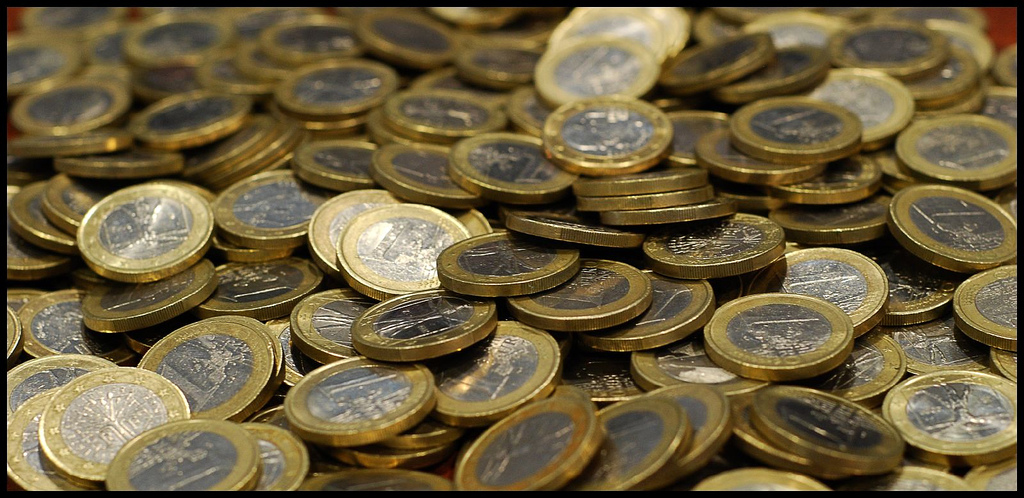
\includegraphics[trim=0.2cm 1.5cm 0.2cm 1.5cm,clip,width=\textwidth]{figuren/rijen/geldstukken.jpg}
\end{center}
\end{figure}



\subsection{Gespaarde kapitaal is een meetkundige rij}
In sectie~\ref{sec:MR}  merkten we op dat het gespaarde kapitaal bij samengestelde intrest per jaar een meetkundige rij is. Bij het derde voorbeeld van sectie~\ref{subsec:voorbeelden_rijen} (op pagina~\pageref{subsec:voorbeelden_rijen}) gaat het om  een meetkundige rij $m_i$ met reden $r=\num{1.06}$ en eerste element $m_0=\num{10000}$. Uit vergelijking~(\ref{eq:rec_mr}) volgt dat een algemeen element $m_j$ dat het gespaarde kapitaal in jaar $j$ weergeeft gelijk is aan 
\begin{equation}
m_j=m_0\cdot r^j=m_0\cdot\num{1.06}^j.
\label{eq:samengest_intrest}
\end{equation}  
We kunnen vergelijking~(\ref{eq:samengest_intrest}) gebruiken om snel te berekenen hoe groot het kapitaal is na bijvoorbeeld 13 jaar:
\[
m_{13}=\num{10000}\cdot\num{1.06}^{13}=\num{21329,28}
\]
We herinneren je even aan vergelijking~(\ref{eq:si}):
\begin{equation}
     K(t)=K(0)\cdot g^{t}=1000\cdot \num{1.07}^{t}
    \label{eq:si2}
\end{equation}
Merk op dat deze vergelijking sterk gelijkt op vergelijking~(\ref{eq:samengest_intrest}). Het belangrijkste verschil bestaat erin dat de index $j$ in vergelijking~(\ref{eq:samengest_intrest}) een geheel getal is, terwijl dat niet zo is in vergelijking~(\ref{eq:si2}). Hieruit besluiten we dat een meetkundige rij met reden $r$ het discrete geval is van een exponentieel groeiproces met groeifactor $r$. 

Wanneer het financi\"ele algebra betreft, maken we geen strikt onderscheid tussen de vergelijking van een meetkundige rij en die van een exponentieel groeiproces. Zo zullen we vergelijking~(\ref{eq:samengest_intrest}) ook gebruiken om te berekenen hoe groot het kapitaal is na bijvoorbeeld anderhalf jaar ($\num{10000}\cdot \num{1.06}^{\num{1.5}}$) of 5 jaar geleden ($\num{10000}\cdot \num{1.06}^{-5}$). 

Voor een exponentieel groeiproces bepaalden we het verband tussen procentuele toename en groeifactor in vergelijking~\eqref{eq:groeifactor_procent}. Op gelijkaardige manier vind je dat de reden van de meetkundige rij bepaald door het gespaarde kapitaal met intrest $i$ gelijk is aan $r=1+i$. 

\subsection{Belangrijke principes uit de financi\"{e}le
algebra}\label{sec.principes}
We brengen enkele belangrijke principes onder de aandacht:
\begin{itemize}
       \item Zichtrekeningen brengen \textit{elke dag} intrest. Als je je spaargeld bijvoorbeeld op 1 februari naar de bank brengt en het terug afhaalt op 21 februari, krijg je voor die 20 dagen ($=20/365$ste van een jaar) intrest.
    \item Kapitaal dat uitstaat tegen samengestelde intrest
      \emph{vermeerdert} in waarde als we verder gaan in de tijd.
       \item Bedragen kan je alleen met elkaar \emph{vergelijken (of optellen)}
       als je ze
       verrekent naar \emph{eenzelfde} tijdstip.
   \end{itemize}

\subsection{Voorbeeld: Samengestelde intrest}
\begin{quote}
Je zet op 1 januari 2012 een bedrag $K$ op een spaarrekening met jaarlijkse intrest \SI{3}{\percent}. Hoe groot moet $K$ zijn opdat er na 3 jaar \euros{100} op de spaarrekening zal staan?
\end{quote}
\subsubsection{Voorbeeld 1: Eerste manier}
\begin{figure}[htbp]
    \centering
\begin{tikzpicture}[x=2.5cm]
\draw[->] (-0.2,0) -- (3.5,0) node [at end, above] {$t$};
\foreach \x/\y in {2012/$K$?,2013/$\cdots$ ,2014/$\cdots$ ,2015/\num{100}}{
	\draw[shift={(\x-2012,0.0)}] (0pt,1pt) -- (0pt,-2pt) node[above=4pt] {\small $\x$};
	\node (\x) [below=4pt] at (\x-2012,0) {\y};
}
\foreach \x/\y in {0/1,1/2,2/3}
	\draw[-latex,red] (\x) to [bend right]  node [below] {$\cdot \num{1,03}$} (\y);
\end{tikzpicture}
    \caption{Welk kapitaal is na drie jaar aangegroeid tot \euros{100} tegen een WR van \SI{3}{\percent}?}
    \label{fig:oef1verdertellen} 
\end{figure}
We stellen de gegevens en het gevraagde voor in figuur~\ref{fig:oef1verdertellen}.

Het gespaarde kapitaal jaar na jaar vormt een meetkundige rij  met volgende kenmerken:
\begin{itemize}
\item begintijdstip 1 januari 2012
\item eerste element $m_0=K$
\item periode 1 jaar
\item reden $r=1+\dfrac{3}{100}=\num{1.03}$
\end{itemize}
zodat het gespaarde kapitaal na $j$ jaar gelijk is aan 
\begin{equation}
m_j=K\cdot \num{1.03}^j.
\label{eq:sam_intrest_vb1}
\end{equation}

Uit het gegeven blijkt dat $m_3=100$. We vullen dit in vergelijking~(\ref{eq:sam_intrest_vb1}) in:
\begin{align*}
100&=K\cdot \num{1.03}^3\\
&\Updownarrow\\
K&=\dfrac{100}{\num{1.03}^3}=\num{96,80}
\end{align*}
Omdat kapitaal dat uitstaat tegen een samengestelde intrest altijd vermeerdert, moet $K$ kleiner zijn dan 100, wat we inderdaad bekomen.

\subsubsection{Voorbeeld 1: Tweede manier}
\label{vb1:2demanier}
Je kan  het vorige voorbeeld ook oplossen door terug te gaan in de tijd. Je neemt dan als begintijdstip van de rij 1 januari 2015. 
\begin{figure}[htbp]
    \centering
\begin{tikzpicture}[x=2.5cm]
\draw[->] (-0.2,0) -- (3.5,0) node [at end, above] {$t$};
\foreach \x/\y in {2012/$K$?,2013/$\cdots$ ,2014/$\cdots$ ,2015/\num{100}}{
	\draw[shift={(\x-2012,0.0)}] (0pt,1pt) -- (0pt,-2pt) node[above=4pt] {\small $\x$};
	\node (\x) [below=4pt] at (\x-2012,0) {\y};
}
\foreach \x/\y in {3/2,2/1,1/0}
	\draw[-latex,red] (\x) to [bend left]  node [below] {$: \num{1,03}$} (\y);
\end{tikzpicture}
    \caption{Welk kapitaal is na drie jaar aangegroeid tot \euros{100} tegen een WR van \SI{3}{\percent}?}
    \label{fig:oef1terugtellen} 
\end{figure}
De rij heeft dan volgende kenmerken:
\begin{itemize}
\item begintijdstip 1 januari 2015
\item eerste element $n_0=100$
\item periode 1 jaar
\item reden $r=1+\dfrac{3}{100}=\num{1.03}$
\end{itemize}
zodat het gespaarde kapitaal na $i$ jaar (sinds 1 januari 2015) gelijk is aan 
\begin{equation}
n_i=100\cdot \num{1.03}^i
\end{equation}
Om het kapitaal op 1 januari 2012 te kennen, moeten we $n_{-3}$ berekenen, dat gelijk is aan 
\[
K=100\cdot \num{1.03}^{-3}=\frac{100}{\num{1.03}^{3}}=\num{96,80}.
\]


\subsubsection{Voorbeeld 2}
\begin{quote}
Op spaarrekening A (jaarlijkse rente \SI{3}{\percent}) stort je op 1 januari 2010 \euros{100}. Op spaarrekening B (jaarlijkse rente \SI{2,5}{\percent}) stort je op 10 januari 2012 \euros{110}. Wanneer is het bedrag op beide spaarrekeningen gelijk?
\end{quote}
\noindent
Voor beide rekeningen vormt het gespaarde kapitaal een meetkundige rij:
\begin{multicols}{2}
\begin{itemize}
\item begintijdstip 1 januari 2010
\item eerste element $a_0=100$
\item periode 1 jaar
\item reden $r=1+\dfrac{3}{100}=\num{1.03}$
\end{itemize}
zodat het gespaarde kapitaal na $j$ jaar gelijk is aan 
\begin{equation}
a_j=100\cdot \num{1.03}^j
\label{eq:sam_intrest_vb2a}
\end{equation}
met $j$ het aantal jaar sinds 1/1/10.
\begin{itemize}
\item begintijdstip 1 januari 2012
\item eerste element $b_0=110$
\item reden $r=1+\dfrac{\num{2.5}}{100}=\num{1.025}$
\end{itemize}
zodat het gespaarde kapitaal na $k$ jaar gelijk is aan 
\begin{equation}
b_k=110\cdot \num{1.025}^k
\label{eq:sam_intrest_vb2b}
\end{equation}
met $k$ het aantal jaar sinds 1/1/12

\end{multicols}
\begin{figure}[htpb]
\centering
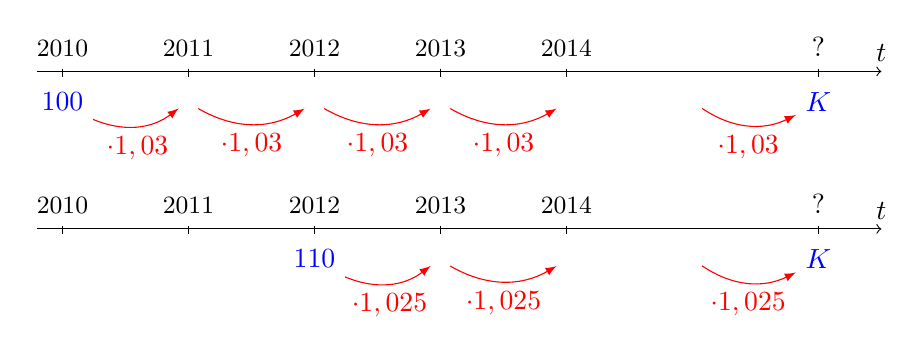
\begin{tikzpicture}[x=1.6cm]
%\draw[dashed] (6,-1) -- (6,3);
%% onderste tijdsas
\draw[->] (-0.2,0) -- (6.5,0) node [at end, above] {$t$};
\foreach \x in {2010,...,2014}{
	\draw[shift={(\x-2010,0.0)}] (0pt,1pt) -- (0pt,-2pt) node[above=4pt] {\small $\x$};
	}
	\draw (6,1pt) -- (6, -2pt) node[above=4pt] {?};
	\node (t12) [below=4pt,blue] at (2,0) {110};
\node (t13)  at (3,-0.4) {};	
\node (t14)  at (4,-0.4) {};
\node (t15)  at (5,-0.4) {};
\node (t16)[below=4pt,blue]  at (6,0) {$K$};
	\draw[-latex,red] (t12) to [bend right]  node [below] {$\cdot \num{1,025}$} (t13);
		\draw[-latex,red] (t13) to [bend right]  node [below] {$\cdot \num{1,025}$} (t14);
			\draw[-latex,red] (t15) to [bend right]  node [below] {$\cdot \num{1,025}$} (t16);
			
%% Deel 2 (bovenste) van de figuur			
\draw[->] (-0.2,2) -- (6.5,2) node [at end, above] {$t$};
\foreach \x in {2010,...,2014}{
	\draw[shift={(\x-2010,2.0)}] (0pt,1pt) -- (0pt,-2pt) node[above=4pt] {\small $\x$};
	}
\draw[shift={(0,2)}] (6,1pt) -- (6, -2pt) node[above=4pt] {?};
\node (tt10) [below=4pt,blue] at (0,2) {100};
\node (tt11)  at (1,1.6) {};	
\node (tt12)  at (2,1.6) {};
\node (tt13)  at (3,1.6) {};
\node (tt14)  at (4,1.6) {};
\node (tt15)  at (5,1.6) {};
\node (tt16)[below=4pt,blue]  at (6,2) {$K$};
\draw[-latex,red] (tt10) to [bend right]  node [below] {$\cdot \num{1,03}$} (tt11);
\draw[-latex,red] (tt11) to [bend right]  node [below] {$\cdot \num{1,03}$} (tt12);
\draw[-latex,red] (tt12) to [bend right]  node [below] {$\cdot \num{1,03}$} (tt13);
\draw[-latex,red] (tt13) to [bend right]  node [below] {$\cdot \num{1,03}$} (tt14);
\draw[-latex,red] (tt15) to [bend right]  node [below] {$\cdot \num{1,03}$} (tt16);
\end{tikzpicture}
\caption{Voorbeeld 2: wanneer zelfde eindbedrag?}
\end{figure}
Bij het oplossen van het vraagstuk moeten we rekening houden met het verschil in begintijdstip. Spaarrekening B heeft altijd 2 jaar minder intrest opgebracht dan rekening A. We moeten dus volgende vergelijking oplossen: Zoek $t$ zodat 
\begin{align*}
a_t&=b_{t-2}\\
&\Updownarrow \\
100\cdot \num{1.03}^t&=110\cdot \num{1.025}^{t-2}\\
&=110\cdot \num{1.025}^{-2}\cdot \num{1.025}^t\\
&\Updownarrow \\
\left(\frac{\num{1.03}}{\num{1.025}}\right)^t&=\frac{110\cdot \num{1.025}^{-2}}{100} \\
&\Updownarrow \\
t&=\frac{\log\left(\dfrac{110\cdot \num{1.025}^{-2}}{100}\right)}{\log\left(\dfrac{\num{1.03}}{\num{1.025}}\right)}
\end{align*}


\subsection{Rente en periode}
Geld wordt niet altijd per jaar belegd. Stel dat je bank je laat kiezen uit twee zichtrekeningen:
\begin{enumerate}
\item Bij zichtrekening A krijg je maandelijks \SI{0,5}{\percent} intrest
\item Bij zichtrekening B krijg je jaarlijks \SI{6}{\percent} intrest
\end{enumerate}
Je hebt \euros{100}. Welk van beide zichtrekeningen is de meest interessante?


We bepalen de meetkundige rijen die horen bij beide zichtrekeningen en het  bedrag dat op de rekening staat na 1 jaar.

\subsubsection{Zichtrekening A}
\begin{itemize}
\item periode: 1 maand
\item reden: $1+\num{0.5}/100=\num{1.005}$
\item beginwaarde $a_0=100$
\end{itemize}
Bijhorende meetkundige rij:
\begin{equation}
a_i=100\cdot \num{1.005}^i \quad \text{met~}i\text{~uitgedrukt~in~maanden.}
\end{equation}
E\'en jaar duurt 12 maanden, dus na 1 jaar staat volgend bedrag op de rekening:
\[
a_{12}=100\cdot \num{1.005}^{12}=106,168
\]


\subsubsection{Zichtrekening B}
\begin{itemize}
\item periode: 1 jaar
\item reden: $1+\frac{6}{100}=1.06$
\item beginwaarde $a_0=100$
\end{itemize}
Bijhorende meetkundige rij:
\begin{equation}
b_j=100\cdot \num{1.06}^j \quad \text{met~}j\text{~uitgedrukt~in~jaren}
\end{equation}
Na 1 jaar staat volgend bedrag op de rekening:
\[
b_1=100\cdot \num{1.06}^1=106
\]

Het bedrag op zichtrekening A is (een beetje) groter, dus zichtrekening A is de meest interessante belegging. Nochtans is de jaarlijkse intrest op zichtrekening B juist 12 keer groter dan de maandelijkse intrest op zichtrekening A. Als de periode verandert met een bepaalde factor, mag je de rente dus \textit{niet} met diezelfde factor vermenigvuldigen. Je moet \emph{eerst} de reden van bijhorende meetkundige rij (met de nieuwe periode) bepalen en van daaruit de rente berekenen. Maak daarbij gebruik van figuur~\ref{fig:periode_factor}.



\subsection{Voorbeeld: Periodiek sparen} 
\label{vb:persparen}

In paragraaf \ref{subsec.Tn} werd volgende formule afgeleid:
\begin{equation}
    T_{n}=t_{0}\cdot \frac{r^{n}-1}{r-1}=t_{0}\cdot \frac{1-r^{n}}{1-r}
    \label{eq:sommr}
\end{equation}
$T(n)$ is de som van $n$ termen van een meetkundige rij met reden
$r$ en eerste term $t_{0}$. In deze paragraaf laten we zien hoe
deze formule gebruikt wordt in financi\"ele algebra. 

\begin{quote}
    Jan wil over 5 jaar een brommer kopen. Daarvoor moet hij over 5
    jaar beschikken over een bedrag van \euros{1750}. Hij begint nu te
    sparen en zet elk \emph{semester} \euros{125} op een rekening met
    samengestelde intrest. De semestri\"{e}le intrest is \SI{5}{\percent}.
    Zal Jan over 5 jaar over voldoende kapitaal beschikken om
    die brommer te kopen?
\end{quote}

\subsubsection{Stap 1: Tijdsas}
We beginnen met de situatie te visualiseren. Daartoe tekenen we een tijdsas waarop we alle gebeurtenissen aanduiden: tijdstippen waarop iets gebeurt, wat er gebeurt (storting), tijdstip waarnaar gerekend moet worden. Dit wordt getoond in figuur~\ref{fig:t1}. 

    \begin{figure}[htb]
            \centering

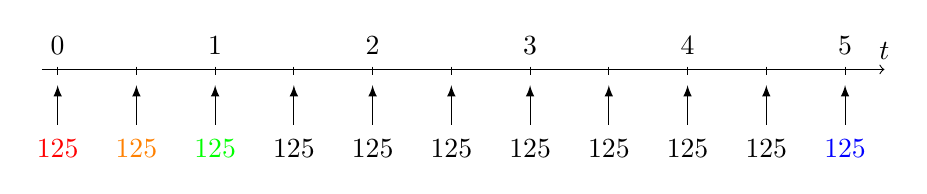
\begin{tikzpicture}[x=1cm]
\draw[->] (-0.2,0) -- (10.5,0) node [at end, above] {$t$};
\foreach \x in {0,...,10}{
	\draw[shift={(\x,0.0)}] (0pt,1pt) -- (0pt,-2pt);
	\draw[shift={(\x,0.0)},-latex] (0,-0.7) -- (0,-0.2);
	}
\foreach \x in {0,...,5}{
	\node at ({\x*2},0.3) {\x};
}
\node[red] at (0,-1) {125};
\node[orange] at (1,-1) {125};
\node[green] at (2,-1) {125};
\foreach \x in {3,...,9}{
	\node at (\x,-1) {125};
}
\node[blue] at (10,-1) {125};
\end{tikzpicture}

        \caption{Semestri\"{e}le stortingen van \euros{125}}
        \label{fig:t1}
    \end{figure}
    \setcounter{tijd}{0}

\subsubsection{Stap 2: Periode en groeifactor bepalen}
In het vraagstuk werken we met samengestelde intrest. Het gespaarde kapitaal neemt elke periode toe met een zelfde groeifactor. Deze factor hangt af van de periode. We moeten beide dus bepalen:
\begin{itemize}
\item de periode is 1 semester
\item de factor is  $r=\num{1.05}$ ($=1+\frac{5}{100}$).
\end{itemize}


\subsubsection{Stap 3: Gespaarde bedragen berekenen}
 Elk semester neemt het gespaarde kapitaal toe met factor $\num{1.05}$. Bovendien stort Jan elke semester \euros{125}. De semestri\"ele rekeninguittreksels van de spaarrekening van Jan zouden er dus kunnen uitzien als in tabel~\ref{tab:persparen}.
\begin{table}[htbp]
\centering
\caption{Gespaarde kapitaal per semester}
\begin{tabular}{cl}
\toprule
semester  & gespaarde kapitaal\\
\midrule
0 & $\textcolor{red}{125}$ \\
1 & $\textcolor{red}{125}\cdot \num{1.05}+\textcolor{orange}{125}$\\
2 & $(\textcolor{red}{125}\cdot \num{1.05}+\textcolor{orange}{125})\cdot \num{1.05}+\textcolor{green}{125}$\\ &$\qquad=\textcolor{red}{125}\cdot \num{1.05}^2+\textcolor{orange}{125}\cdot \num{1.05}+\textcolor{green}{125}$\\
3 & $(\textcolor{red}{125}\cdot \num{1.05}^2+\textcolor{orange}{125}\cdot \num{1.05}+\textcolor{green}{125})\cdot \num{1.05}+125$\\&$\qquad=\textcolor{red}{125}\cdot \num{1.05}^3+\textcolor{orange}{125}\cdot \num{1.05}^2+\textcolor{green}{125}\cdot \num{1.05}+125$\\
\dots & \dots \\
10 & $\textcolor{red}{125}\cdot \num{1.05}^{10}+\textcolor{orange}{125}\cdot \num{1.05}^9+\dots+125\cdot \num{1.05}+\textcolor{blue}{125}$\\
\bottomrule
\end{tabular}
\label{tab:persparen}
\end{table}

De som na 10 semesters kan je ook als volgt bekijken: 
\begin{itemize}
\item de \euros{\textcolor{red}{125}} die gestort worden op semester 0 staan 10 semesters op de rekening. Hun aandeel in het gespaarde kapitaal is gelijk aan $125\cdot \num{1.05}^{10}$
\item de \euros{\textcolor{orange}{125}} die gestort worden op semester 1 staan 9 semesters op de rekening. Hun aandeel in het gespaarde kapitaal is gelijk aan $125\cdot \num{1.05}^{9}$
\item \dots
\item de laatste \euros{\textcolor{blue}{125}} staan nog maar net op de rekening en hebben nog geen intrest opgebracht. Hun aandeel is gelijk aan 125.
\end{itemize}
In wat volgt zullen we het gespaarde bedrag steeds op deze manier berekenen. We gebruiken de figuur daartoe als hulpmiddel. Bij elk bedrag tekenen we een pijl die aangeeft met welke factor het bedrag vermenigvuldigd moet worden. 


    \begin{figure}[htb]
            \centering
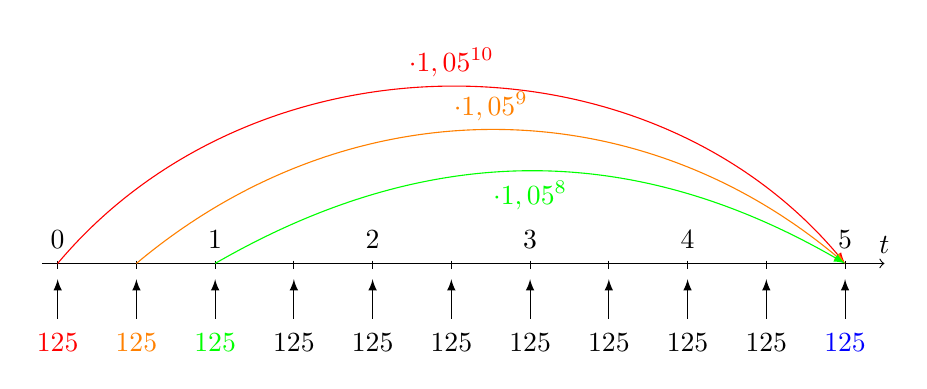
\begin{tikzpicture}[x=1cm]
\draw[->] (-0.2,0) -- (10.5,0) node [at end, above] {$t$};
\foreach \x in {0,...,10}{
	\draw[shift={(\x,0.0)}] (0pt,1pt) -- (0pt,-2pt);
	\draw[shift={(\x,0.0)},-latex] (0,-0.7) -- (0,-0.2);
	}
\foreach \x in {0,...,5}{
	\node at ({\x*2},0.3) {\x};
}
\node[red] at (0,-1) {125};
\node[orange] at (1,-1) {125};
\node[green] at (2,-1) {125};
\foreach \x in {3,...,9}{
	\node at (\x,-1) {125};
}
\node[blue] at (10,-1) {125};
\draw[-latex,red] (0,0) to  [out=50,in=130]  node [above] {$\cdot \num{1,05}^{10}$} (10,0);
\draw[-latex,orange] (1,0) to  [out=40,in=140]  node [above] {$\cdot \num{1,05}^{9}$} (10,0);
\draw[-latex,green] (2,0) to  [bend left]  node [below] {$\cdot \num{1,05}^{8}$} (10,0);
\end{tikzpicture}
        \caption{Semestri\"{e}le stortingen van \euros{125}}
        \label{fig:tt1}
    \end{figure}
    \setcounter{tijd}{0}


\subsubsection{Stap 4: Som van elementen van een meetkundige rij}
In de vorige stap berekenden we dat Jan volgend bedrag gespaard zal hebben:
\begin{equation}
K= 125\cdot \num{1.05}^{10}+125\cdot \num{1.05}^9+\dots+125\cdot \num{1.05}+125
\label{eq:som_vb2}
\end{equation}
Wanneer we de termen van de som bekijken, merken we op dat het elementen zijn van een meetkundige rij met volgende kenmerken:
\begin{itemize}
\item eerste term $t_0=125\cdot \num{1.05}^{10}$
\item reden $r=\dfrac{t_1}{t_0}=1/\num{1.05}$
\item aantal\footnote{Opgepast: dit is een bron van
    fouten. Tussen 0 en 10 liggen 10 stappen, maar het zijn in totaal 11
    getallen. Kijk dus in oefeningen altijd goed na of je je niet 1
    eenheid vergist!} elementen: 11
\end{itemize}
Als we gebruik maken van vergelijking~\eqref{eq:sommr} vinden we eenvoudig
\begin{equation}
K=125\cdot\num{1.05}^{10}\cdot \dfrac{1-\left(\frac{1}{\num{1.05}}\right)^{11}}    {1-\frac{1}{\num{1.05}} }
\end{equation}

Het staat je vrij om de termen van som~(\ref{eq:som_vb2}) te herschikken, bijvoorbeeld
\begin{equation}
K=125 +125\cdot \num{1.05}+\dots+125\cdot \num{1.05}^9+125\cdot \num{1.05}^{10}
\label{eq:som_vb2_anders}
\end{equation}
De reden is dan geen breukgetal meer:
\begin{itemize}
\item eerste term $s_0=125$
\item reden $r=\dfrac{s_1}{s_0}=\num{1.05}$
\item aantal termen: 11
\end{itemize}
zodat de somformule een eenvoudigere uitdrukking is 
\begin{equation}
K=125\cdot \frac{1-\num{1.05}^{11}} {1-\num{1.05}}
\label{eq:som_vb2bis}
\end{equation}
Reken zelf uit dat vergelijking~(\ref{eq:som_vb2}) en (\ref{eq:som_vb2bis}) aan mekaar gelijk zijn. 

\subsubsection{Stap 5: Antwoord formuleren}
Als je vergelijking~(\ref{eq:som_vb2}) berekent, vind je $K=1776$. Jan heeft  meer gespaard dan nodig en dus kan hij de brommer kopen.

\subsection{Periodiek sparen en lenen: Algemene werkwijze}

We veralgemenen de werkwijze die we in de vorige sectie uitgerold hebben. 

\subsubsection{1. Tijdsas}
Stel de gegevens schematisch voor op een tijdsas.
\begin{itemize}
\item Geef de as een richting (pijl) en noteer in welke tijdseenheid je
werkt (bijvoorbeeld jaren of maanden).
\item Je mag de as onderbreken met puntjes.
\item Duid aan wat er wanneer gebeurt: op welke tijdstippen wordt er geld
gestort/afgehaald? 	
\item Duid het tijdstip $T$ aan waarnaar je rekent.
\end{itemize}

\subsubsection{2.	Periode en reden}
Noteer de periode waarin je de berekeningen zal doen. Bereken de bijbehorende reden. Vermijd afrondingen. Werk liever met $\sqrt{\num{1.05}}$ dan met $\num{1.02469507}$.

\subsubsection{3.	Gespaarde bedragen}
Duid op de tijdsas met behulp van pijlen aan hoe de bedragen veranderen als je ze omrekent naar het tijdstip $T$.

\subsubsection{4. Som}
In de meeste opgaven moet je een som berekenen.
\begin{itemize}
\item Schrijf de som volledig uit.  Dit wil zeggen: eerste, tweede en laatste
term;
\item 	Indien je de som maakt van elementen van een meetkundige rij,
noteer dan
\begin{itemize}
\item het eerste element $t_0$; 
\item de reden $r$; 
\item het aantal elementen van de rij.
\end{itemize}
\item 	Pas de somformule toe. 	
\item Bereken de waarde van de som bijvoorbeeld met Scilab.
\end{itemize}

\subsubsection{5. Antwoord}
Formuleer het antwoord.


\subsection{Voorbeeld : Lening}
Lenen en (periodiek) sparen zijn  gelijkaardige processen: je zet op regelmatige tijdstippen geld opzij. Het belangrijke verschil is dat je bij lenen het totaalbedrag op voorhand ter beschikking hebt. Dit resulteert in een verschillende werkwijze bij oefeningen over sparen en lenen: bij sparen berekenen we de waarde van een bedrag in de toekomst; bij lenen kijken we hoeveel een bedrag een tijdje geleden waard was. 
\begin{quote}
    We lenen een bedrag van \euros{5\,000} bij de bank voor de aankoop
    van een auto. We komen overeen dat bedrag terug te betalen over
    een periode van 10 jaar, door middel van jaarlijkse \emph{constante}
    aflossingen. We nemen aan dat de jaarlijkse rente over die periode \SI{5}{\percent} is.
    De eerste afbetaling doen we \'{e}\'{e}n jaar na aankoop. Welk
    bedrag $K$ moeten we jaarlijks afbetalen?
\end{quote}
Er zijn twee verschillen met  sectie~\ref{vb:persparen}: het vraagstuk gaat over lenen \'en het eindbedrag is gekend en niet het bedrag van de jaarlijkse stortingen.

We volgen de algemene werkwijze, ervan uitgaand dat de bank
geen verlies en geen winst mag maken. Geld wordt ook niet meer in
de kous gestopt maar wordt uitgezet tegen samengestelde intrest.

\subsubsection{Stap 1: Tijdsas}
We tekenen een tijdsas, figuur~\ref{fig:t2}, waarop we de 10 jaren uitzetten.
    Onder tijdstip $t=1$ en alle volgende duiden we het bedrag $T$ aan.
    Boven tijdstip $t=0$ zetten we het ontleende bedrag $5\,000$.
    \begin{figure}[htb]
            \centering
            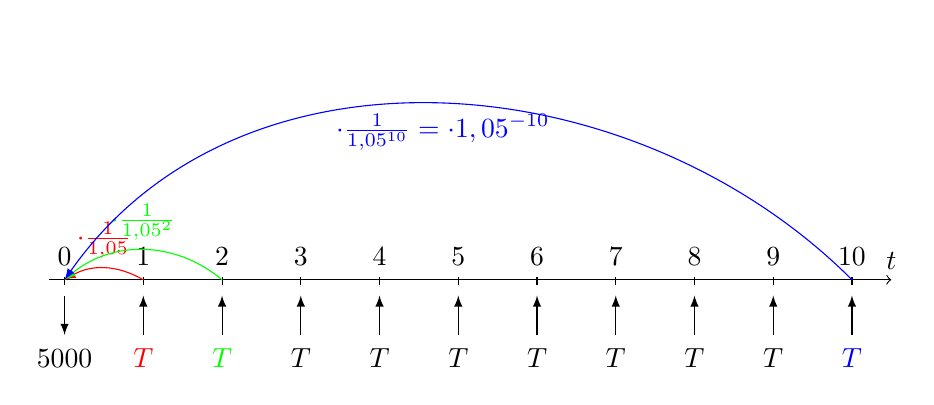
\begin{tikzpicture}[x=1cm]
\draw[->] (-0.2,0) -- (10.5,0) node [at end, above] {$t$};
\foreach \x in {0,...,10}{
	\draw[shift={(\x,0.0)}] (0pt,1pt) -- (0pt,-2pt);
	\node at ({\x},0.3) {\x};
	}
\foreach \x in {1,...,10}{
	\draw[shift={(\x,0.0)},-latex] (0,-0.7) -- (0,-0.2);
}
\draw[latex-] (0,-0.7) -- (0,-0.2);
\node at (0,-1) {\num{5000}};
\node[red] at (1,-1) {$T$};
\node[green] at (2,-1) {$T$};
\foreach \x in {3,...,9}{
	\node at (\x,-1) {$T$};
}
\node[blue] at (10,-1) {$T$};
\draw[-latex,red] (1,0) to  [out=150,in=30]  node [above] {$\cdot \frac{1}{ \num{1,05}}$} (0,0);
\draw[-latex,green] (2,0) to  [out=140,in=40]  node [above] {$\cdot \frac{1}{ \num{1,05}^{2}}$} (00,0);
\draw[-latex,blue] (10,0) to  [out=135,in=55]  node [below] {$\cdot \frac{1}{ \num{1,05}^{10}}=\cdot \num{1,05}^{-10}$} (0,0);
\end{tikzpicture}
        \caption{Tijdsas voor de autolening}
        \label{fig:t2}
    \end{figure}
    \setcounter{tijd}{0}

\subsubsection{Stap 2: Periode en reden}
\begin{itemize}
\item periode: 1 jaar
\item rente is \SI{5}{\percent}, dus $r=\num{1.05}$
\end{itemize}

\subsubsection{Stap 3: Gespaarde bedragen}
     Elk terugbetaald bedrag $T$ draagt bij tot het ontleende kapitaal. Omdat het ene bedrag later terugbetaald wordt dan het ander, is die bijdrage tot het kapitaal steeds verschillend. We moeten voor elke bijdrage berekenen hoeveel die waard was bij aankoop van de auto. We doen dit zoals aangegeven op blz.~\pageref{vb1:2demanier}.
     \begin{itemize}
\item het bedrag dat 1 jaar na aankoop terugbetaald werd (uitgerekend naar het referentietijdstip $t=0$): $\textcolor{red}{T\cdot \num{1.05}^{-1}}$
\item 2 jaar na aankoop: $\textcolor{green}{T\cdot \num{1.05}^{-2}}$
\item \dots
\item 10 jaar na aankoop: $\textcolor{blue}{T\cdot \num{1.05}^{-10}}$
\end{itemize}
Op de tijdsas duiden we dat aan door pijlen te trekken van de verschillende `terugbetaalmomenten' naar het begintijdstip toe. Omdat we teruggaan in de tijd, moeten we vermenigvuldigen met een \emph{negatieve} macht van de reden (of, wat op hetzelfde neerkomt, delen door de positieve macht).

\subsubsection{Stap 4: Som}
Het geleende bedrag is gelijk aan
\begin{equation}
5\,000=\textcolor{red}{T\cdot \num{1.05}^{-1}}+\textcolor{green}{T\cdot \num{1.05}^{-2}}+\dots+\textcolor{blue}{T\cdot \num{1.05}^{-10}}s
\end{equation}
Dit is een som van elementen van een meetkundige rij met volgende kenmerken:
\begin{itemize}
\item eerste term $t_0=T\cdot \num{1.05}^{-1}$
\item reden $r=\dfrac{t_1}{t_0}=\num{1.05}^{-1}$
\item aantal termen $n=10$
\end{itemize}
De som is dus gelijk aan
\begin{equation}
5\,000=T\cdot \num{1.05}^{-1}\cdot \frac{1-\left(\num{1.05}^{-1}\right)^{10}}{1-\num{1.05}^{-1}}
\end{equation}
Uit deze eerstegraadsvergelijking kunnen we $T$ oplossen:
\begin{equation}
T=\frac{5\,000}{ \num{1.05}^{-1}\cdot \dfrac{1-\left(\num{1.05}^{-1}\right)^{10}}{1-\num{1.05}^{-1}}}=\num{647.5}
\end{equation}

\subsubsection{Stap 5: Antwoord}
De lening is volledig terugbetaald
    door 10 opeenvolgende jaren \euros{\num{647.5}} te betalen aan de bank.


